\documentclass[t,xcolor=dvipsnames]{beamer}
\usepackage{epsfig}
\usepackage{inputenc}
\usepackage{verbatim}
\usepackage{alltt}
\usepackage{ulem}
\usetheme[height=7mm]{Rochester}
\setbeamertemplate{blocks}[rounded]

\title[]{A look at Parsoid internals}
\author{Subramanya Sastry (Subbu) \\Gabriel Wicke}
\institute{
  {\bf Wiki}: http://www.mediawiki.org/wiki/Parsoid \\
  {\bf Team}: Arlo, Gabriel, Marc, Scott, Subbu\\
  {\bf Alumnus}: Mark Holmquist
}
\date{April 15, 2014}

%----- New commands for inline wikitext/HTML/commands -----
\newcommand{\WT}[2][\small]{\color{blue} #1{\tt #2}}
\newcommand{\TOK}[2][\small]{\color{teal} #1{\tt #2}}
\newcommand{\HTML}[2][\small]{\color{brown} #1{\tt #2}}
\newcommand{\BASH}[2][\small]{\color{Mahogany} #1{\tt \%} #2}

%----- New environments for block wikitext/HTML -----
\newenvironment{wikitext}[1][\small]%
{\begin{alltt}\bgroup\color{blue}#1}%
{\egroup\end{alltt}}

\newenvironment{html}[1][\small]%
{\begin{alltt}\bgroup\color{brown}#1}%
{\egroup\end{alltt} }

\newenvironment{token}[1][\small]%
{\begin{alltt}\bgroup\color{teal}#1}%
{\egroup\end{alltt} }

\begin{document}

% --- TOC control ----
\AtBeginSection[]{
  \begin{frame}<beamer>
    \frametitle{Outline}
    \tableofcontents[
        currentsection,
        sectionstyle=show/shaded,
        subsectionstyle=hide]
  \end{frame}
}
\AtBeginSubsection[]{
  \begin{frame}<beamer>
    \frametitle{Outline}
    \tableofcontents[
        currentsection,
        currentsubsection,
        sectionstyle=show/shaded,
        subsectionstyle=show/shaded/hide]
  \end{frame}
}

% --- title ---
\begin{frame}
\titlepage
{\tiny Talk prepared using LaTeX, Beamer and InkScape}
\end{frame}

\section{Introduction}

% --- Intro ---
\begin{frame}{Introduction: What is Parsoid?}
\begin{itemize}
\item Service that converts between wikitext and HTML5 + RDFa. \\
      Spec @ {\url mediawiki.org/wiki/Parsoid/MediaWiki\_DOM\_spec}
\item Written in Javascript, running on node.js
\item Provides a relatively simple API: \\
\only<2-3>{
\vspace{1ex}
\emph{Wikitext to HTML} \\
\hspace{3ex}{\color{blue} {\tt POST /enwiki/Main\_Page}} \\
\hspace{3ex}{\color{blue} {\tt wt: "foo"}} \\
\vspace{2ex}
\hspace{3ex}{\color{brown} {\tt <i>foo</i>}} \\
}%
\only<3>{
\vspace{1ex}
\emph{HTML to wikitext} \\
\hspace{3ex}{\color{blue} {\tt POST /enwiki/Main\_Page}} \\
\hspace{3ex}{\color{blue} {\tt HTML: <i>foo</i>}} \\
\vspace{2ex}
\hspace{3ex}{\color{brown} {\tt "foo"}} \\
}%
\only<4> {
\vspace{1ex}
\emph{Fetch HTML for a page} \\
\hspace{3ex}{\color{blue} {\tt GET /enwiki/Main\_Page}} \\
\vspace{2ex}
\hspace{3ex}{\color{brown} {\tt <html ...> .. </html>}}
\vspace{1ex}
\item {\footnotesize Visit {\url mediawiki.org/wiki/Parsoid\#The\_Parsoid\_web\_API}}
}%
\only<5>{
\item Provides convenient command-line utilities\\
{\BASH {\tt node parse --wt2html < wikitext}}\\
{\BASH {\tt node parse --html2wt < html}}\\
{\BASH {\tt node parse --wt2wt < wikitext}}\\
{\BASH {\tt node parse --html2html < html}}\\
{\BASH {\tt node parse --help}} {\small for more}\\
}
\end{itemize}
\end{frame}

\begin{frame}{Introduction: Who uses Parsoid?}
\begin{itemize}
  \item Visual Editor uses it both ways
  \item Flow uses it to support wikitext editing in html discussions.
  \item PDF rendering, Mobile, Kiwix use rendered html.
  \item Content translation uses it both ways to support translation between wikis.
  \item Gadgets, bots? ...
  \item Full list @ {\url mediawiki.org/wiki/Parsoid/Users}
\end{itemize}
\end{frame}

\section{What makes this challenging?}

% --- What are the challenges? ---
\begin{frame}{What makes this challenging?}

{\bf HTML should convert back to wikitext without ``dirty diffs''}
\begin{itemize}
  \item {\WT* foo} and {\WT *foo} are different even though they map to the same HTML DOM.
  \item
  \begin{wikitext}
  <ref name=`foo'>..</ref>\\
  <ref name = foo>..</ref>\\
  <REF name="foo">..</REF>
  \end{wikitext}
  %\item Requires Parsoid to maintain a 1-1 mapping between wikitext and html.
  \item Requires Parsoid to serialize unmodified HTML to the exact same wikitext.
\end{itemize}

% --- {\bf Parsoid handles this by:}
% --- \begin{itemize}
% ---    \item Mapping wikitext substrings to DOM subtrees.
% ---    \item Maintaining some state
% --- \end{itemize}
\end{frame}

% --- What are the challenges? ---
\begin{frame}{What makes this challenging?}

{\bf Overloaded syntax makes for complex semantics}

\begin{itemize}
\small
\item Simple links:
  \begin{wikitext}[\small]
  [[Foo]], [[Foo|Foo]], [[Foo|bar]]
  \end{wikitext}
\item Link prefixes and suffixes/trails/tails:
  \begin{wikitext}[\small]
  [[Foo|bar]]s, Pre[[fix|Suf]]fix
  \end{wikitext}
\item Interwiki links:
  \begin{wikitext}[\small]
  [[fr:Interwiki]], [[wikt:fr:Blah]]
  \end{wikitext}
\item Templated links:
  \begin{wikitext}[\small]
  [[\{\{echo|Foo\}\}|\{\{echo|bar\}\}]]s
  \end{wikitext}
\item Images:
  \begin{wikitext}[\small]
  [[Image:Foo.jpg|caption]], [[Image:Foo.jpg|thumb|300px]],
  [[File.Foo.jpg|thumb|right|<table>..</table>]]
  \end{wikitext}
\item External links, URL links, Magicword links
  \begin{wikitext}[\small]
  [http://www.mediawiki.org MW], http://google.com, \\
  ISBN 0123456789, PMD something, RFC 1034
  \end{wikitext}
\end{itemize}

\end{frame}

% --- What are the challenges? ---
\begin{frame}{What makes this challenging?}

{\bf Wikitext templates are string-based: no DOM semantics}
\begin{itemize}
  \item Template output can have non-local effects on DOM structure.
    \begin{wikitext}
    foo \{\{echo|<div>\}\} a lot of wikitext here </div>
    \end{wikitext}
  \item Requires all templates to be expanded first before DOM can be built.
  \item How do you edit this in a HTML editor like VisualEditor? Transclusion output cannot be mapped to any DOM node.
\end{itemize}

{\bf Some pages can have 100s of transclusions}
\begin{itemize}
  \item If expansions are done sequentially, parsing can be very inefficient.
\end{itemize}

% --- {\bf Parsoid handles this by:}
% --- \begin{itemize}
% ---   \item Parsoid recovers by expanding template scope to a DOM subtree.
% ---   \item In the above example, {\WT echo} template output is expanded to {\WT a lot of wikitext here}.
% ---   \item More later with an example.
% --- \end{itemize}
\end{frame}

% --- What are the challenges? ---
\begin{frame}{What makes this challenging?}

{\bf There is no ``invalid'' wikitext}

\begin{itemize}
  \item
    \begin{wikitext}
      <div><small>foo</div> \\
      \{| \\
      |- This text is dropped \\
      | 2.7183 || i || 3.1415 || 1 \\
      |\}
    \end{wikitext}
  \item
    \begin{wikitext}
      <table> \\
      This text will move out of the table \\
      <tr><td>foo</td></table>
    \end{wikitext}
  \item
    \begin{wikitext}
    <div title="foo'>Mismatched quotes</div>
    \end{wikitext}
  \item
    \begin{wikitext}
    <i><b>overlapping</i>tags</b>
    \end{wikitext}
  \item
    %-- Explicit [\small] so that the wikilink is not interpreted
    %-- as an argument to the wikitext environment.
    \begin{wikitext}[\small]
    [[Foo.jpg|thumb|caption 1|caption 2 will be lost]]
    \end{wikitext}
\end{itemize}

% --- {\bf Parsoid handles this by:}
% --- \begin{itemize}
% ---   \item Maintains information about fixups
% --- \end{itemize}
\end{frame}

\section{Parsoid pipeline}

% --- 10K feet overview ---
\begin{frame}{Parsoid pipeline: 10,000 feet view}
\vspace*{-0.3in}
\begin{center}

%-- wt2html --
\begin{figure}
  \hspace*{-0.3in}
  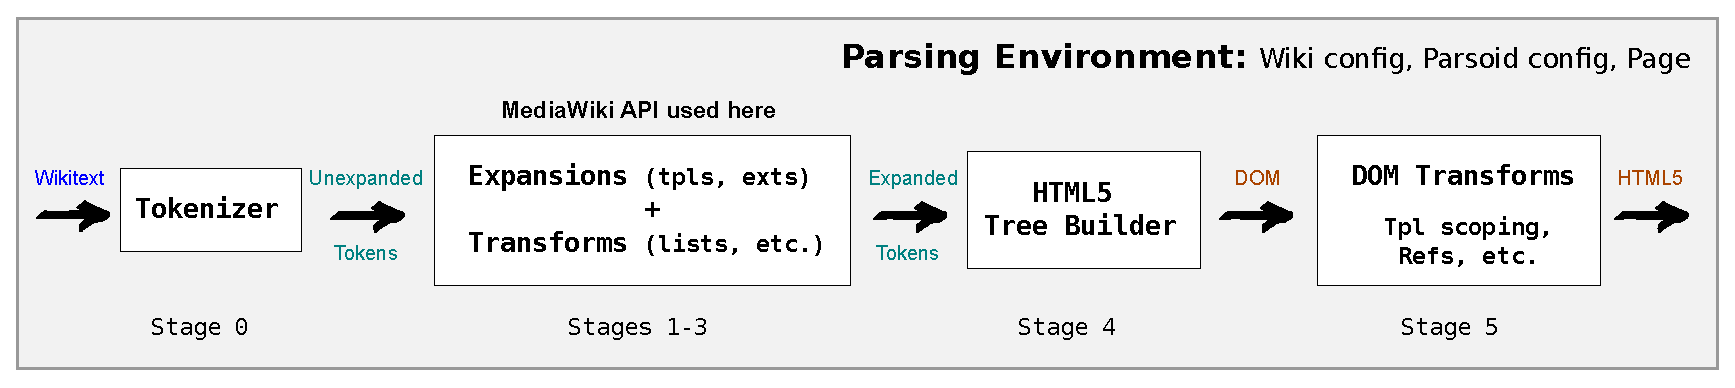
\epsfig{file=figs/parsoid.wt2html.eps,scale=0.42}\\
  {\small Wikitext to HTML (wt2html) transformation}
\end{figure}
\end{center}

%-- pipelines --
\only<2>{
\footnotesize
\vspace{2ex}
\begin{tabular}{|l|c|l|l|} \hline
\footnotesize
{\bf Pipeline}            & {\bf Stages} & {\bf Input} & {\bf Output} \\ \hline
text/mediawiki/full       & 0-5 & Wikitext   & HTML \\
text/mediawiki            & 0-2 & Wikitext   & Expanded Tpls \\
%tokens/mediawiki          & 1-2 & Unexpanded & Expanded Tpls \\
%                          &     & Tokens     & \\
tokens/mediawiki/expanded & 3-5 & Expanded Tpls  & HTML \\ \hline
\end{tabular}

\vspace{3ex}

\begin{itemize}
\item Some pipeline types used by Parsoid
\item Other pipelines can be constructed by hooking up modules and callbacks
\end{itemize}
}
%-- html2wt --
\only<3>{
\begin{center}
  \begin{figure}
    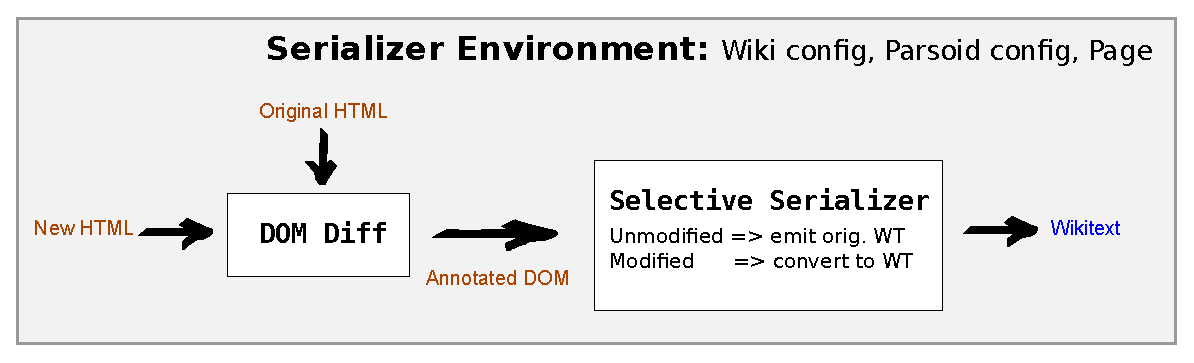
\epsfig{file=figs/parsoid.html2wt.eps,scale=0.42}\\
    {\small HTML to Wikitext (html2wt) transformation}
  \end{figure}
\end{center}
}

\end{frame}

%--- Tokenizer ---
 \subsection{Tokenizer}
 
\begin{frame}{Tokenizer: Short overview}
\begin{itemize}
\item Uses a PEG parser.
\item Parses the context-free aspects of the syntax.
\item Not possible to parse all wikitext constructs to final output because of context-sensitivity and transclusions.
\item Token stream transformations and DOM passes (stages 1-5) handle context sensitive parts.
\end{itemize}
\end{frame}

%--- Example ---
\subsection{Example}

\begin{frame}{Example}
\vspace*{-0.3in}
\begin{figure}
  \hspace*{-0.3in}
  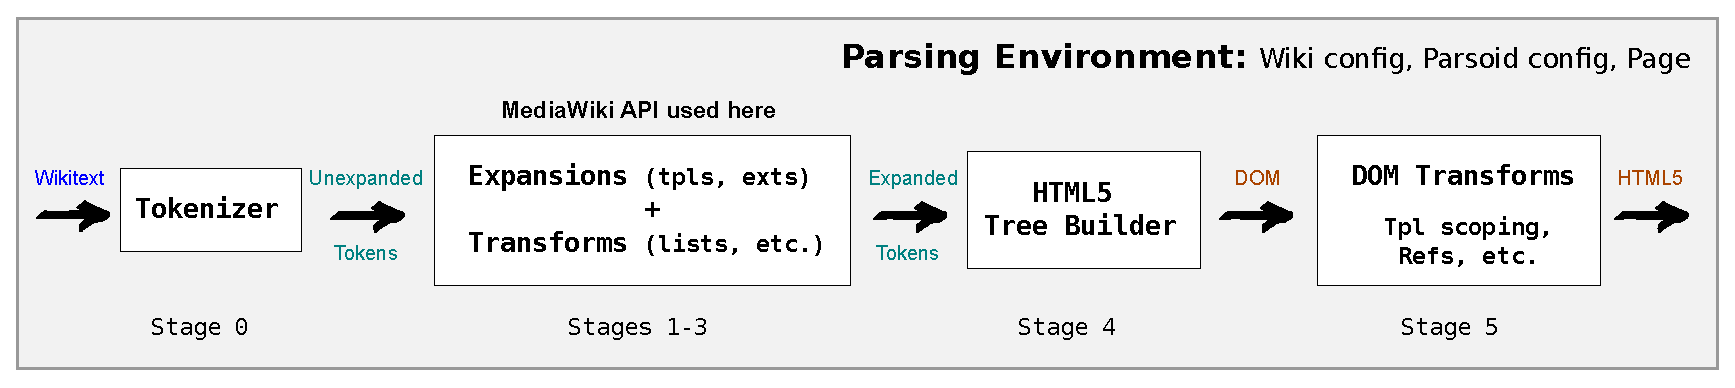
\epsfig{file=figs/parsoid.wt2html.eps,scale=0.42}
\end{figure}
\vspace*{-0.15in}

\emph{Wikitext}
\only<1-7>{
  \begin{wikitext}
  a\\
  *\{\{echo|b\}\}
  \end{wikitext}
}
\only<8>{
  \begin{wikitext}
  a\\
  *\{\{echo|[[Foo]]\}\}
  \end{wikitext}
}

\only<2>{
  \emph{Tokenizer Output} \\
  {\BASH {\tt node parse --trace peg-tokens < wikitext}}$^{*}$
  \begin{token}
  "a", <NL>, <LI:*>, <TPL:echo:["b"]>, <NL>, <EOF>
  \end{token}

  {\color{gray}{\scriptsize $*$ Trace output is simplified and reformatted.}}
}

\only<3>{
  \emph{Expanded Tokens} \\
  {\BASH {\tt node parse --trace html < wikitext}}
  \begin{token}
  <p>, "a", </p>, <NL>, <ul>, <li>, <tpl-start:1>, "b",\\
  <tpl-end:1>, </li>, </ul>, <NL>, <EOF>
  \end{token}
}

\only<4>{
  \emph{Simplified DOM$^{*}$ after some initial passes} \\
  {\BASH {\tt node parse --dump dom:pre-dsr < wikitext}}
  \begin{html}
  <body><p>a</p>\\
  <ul><li><meta typeof="mw:Transclusion" about="\#mwt1">b<meta typeof="mw:Transclusion/End" about="\#mwt1"></li></ul>\\
  </body>
  \end{html}
  \vspace*{-0.1in}
  {\color{gray}$*$ \scriptsize Nodes have addl. information in a data-parsoid attribute not shown here.}
}

\only<5>{
  \emph{HTML (Reformatted)}
  \begin{html}[\footnotesize]
  <body data-parsoid='\{"dsr":[0,14,0,0]\}'>\\
  <p data-parsoid='\{"dsr":[0,1,0,0]\}'>a</p>\\
  <ul data-parsoid='\{"dsr":[2,13,0,0]\}'>\\
  <li data-parsoid='\{"dsr":[2,13,1,0]\}'>\\
  <span about="\#mwt1" typeof="mw:Transclusion" data-mw=".."\\ data-parsoid="\{..\}">b</span></li></ul></body>
  \end{html}
}

\only<6-8>{
  \emph{data-mw of the transclusion span}
  \begin{html}
  \{"parts":[\{\\
    "template":\{ \\
      "target":\{"wt":"echo","href":"./Template:Echo"\}, \\
      "params":\{"1":\{"wt":% --- suppress whitespace ---
      \only<1-7>{"b"}%
      \only<8>{"[[Foo]]"}%
      \only<7>{, {\color{BrickRed}"html": "b"}}%
      \only<8>{, {\color{BrickRed}"html": "<a href=..>Foo</a>"}}%
     \}\} \\
     \}\}]\}
  \end{html}
}
\end{frame}

\subsection{Stages 1-3}

% ---- Expansions ----
\begin{frame}{Zooming in: Stages 1-3: Template expansions, etc.}
\vspace*{-0.1in}
\begin{figure}
  \hspace*{-0.2in}
  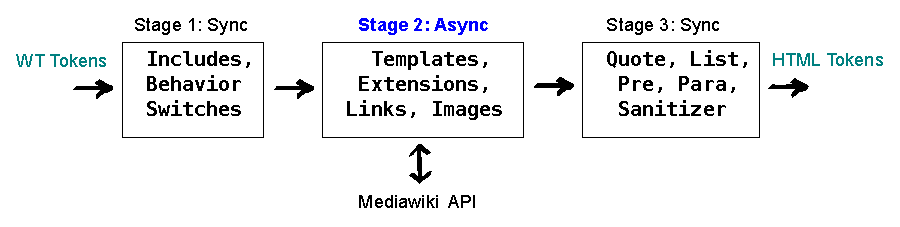
\epsfig{file=figs/expansion.eps,scale=0.75}
\end{figure}

\only<2->{
\begin{columns}
  \begin{column}{0.20\textwidth}
    %--- Use the main running example (with enhancement) --
    \emph{Wikitext}
    \begin{wikitext}
      a\\
      *\{\{echo|b\}\}
      <noinclude>
      \{\{Docs\}\}
      </noinclude>
    \end{wikitext}
    \only<5>{
      \begin{wikitext}
        \{\{echo|[[Foo]]\}\}\\
        \{\{Infobox|..\}\}
      \end{wikitext}
    }
  \end{column}

  \begin{column}{0.80\textwidth}
  \only<2-3>{
    \emph{Unexpanded Tokens}
    \begin{token}
     .. <LI:*>, <TPL:echo:["b"]>, <NL>, <noinclude>, <TPL:Docs:[]>, </noinclude> ..
    \end{token}
    \only<3>{
      \emph{Tokens after Stage 1}
      \begin{token}
       .. <LI:*>, <TPL:echo:["b"]>, <NL>, <placeholder-for-RTing> ..
      \end{token}
    }
  }% --- suppress whitespace ---
  \only<4>{
    \emph{Expansion of template token: {\TOK {\tt <TPL:echo:["b"]>}}}
    \vspace*{0.1in}
    \begin{itemize}
      \item Query mediawiki API for expanded wikitext: {\WT b}
      \item Parse expanded wikitext in a {\bf new pipeline}
            \vspace*{-0.05in}
            \begin{token} "b", <EOF> \end{token}
      \item Wrap {\TOK tpl-start} and {\TOK tpl-end} tokens around it
            \vspace*{-0.05in}
            \begin{token}<tpl-start:1>, "b", <tpl-end:1>\end{token}
      \item Splice tokens into the main token stream
            \vspace*{-0.05in}
            \begin{token}.. <LI:*>, <tpl-start:1>, "b", <tpl-end:1>, <NL> ..\end{token}
    \end{itemize}
  }% --- suppress whitespace ---
  \only<5>{
    \emph{Expansion of template tokens}
    \vspace*{0.1in}
    \begin{itemize}
      \item Template tokens are processed asynchronously
      \item Multiple concurrent requests to MW API
      \item Token buffers ensure tokens are spliced in order
    \end{itemize}
  }

  \end{column}
\end{columns}
}
\end{frame}

\subsection{Stage 3 Transformations}

%-- Stage 3 transformations --
\begin{frame}{Stage 3: Transformations}

\vspace*{-0.1in}
\begin{figure}
  \hspace*{-0.2in}
  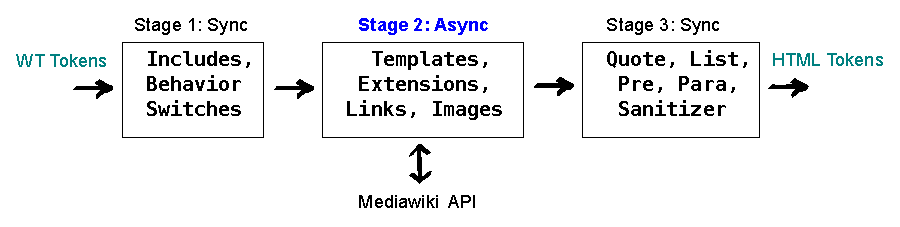
\epsfig{file=figs/expansion.eps,scale=0.75}
\end{figure}

\begin{itemize}
\item Stage 3 transformations run after all templates and extensions have been expanded.
\item Quote Handler is more or less a straight port of the PHP parser's handler.
\item Sanitizer is also a port of the PHP sanitizer.
\item List, Indent Pre, and Paragraph transformers use state machines to transform the token stream.
\end{itemize}

\end{frame}

%-- Sample stage 3 handler --
\begin{frame}{Stage 3: Indent-Pre Handler}
\begin{itemize}
\small
\item Slice of the state machine shown below.
\begin{center}
\vspace{1ex}
\begin{tabular}{|l|c|l|l|} \hline
\small
{\bf Start} & {\bf Token} & {\bf End} & {\bf Action} \\ \hline
SOL & nl/eof & SOL    & Emit \\
    & sol-tr & SOL    & Buffer1 \\
    & ws     & PRE    & Buffer2 \\
    & other  & IGNORE & Emit \\ \hline
PRE & nl/eof & SOL    & Emit \\
    & html-block-tag  & IGNORE & Emit \\
    & wt-table-tag    & IGNORE & Emit \\
    & sol-tr & PRE    & Buffer3 \\
    & other  & PRE-COLLECT & Buffer4 \\ \hline
 ... & ... & ... & ... \\ \hline
\end{tabular}
\vspace{1ex}
\end{center}
\item SOL = Start of Line; WS = white space; Buffer1,2,3,4: buffering depending on state and token
\item Handles single-line, multi-line pres, interaction with SOL-transparent tokens (comments, noinclude, categories), etc.
\end{itemize}

\end{frame}

%--- HTML building ---
\subsection{Stage 4: HTML Building}
\begin{frame}{Stage 4: HTML Building}
\vspace*{-0.3in}
\begin{center}
\begin{figure}
  \hspace*{-0.3in}
  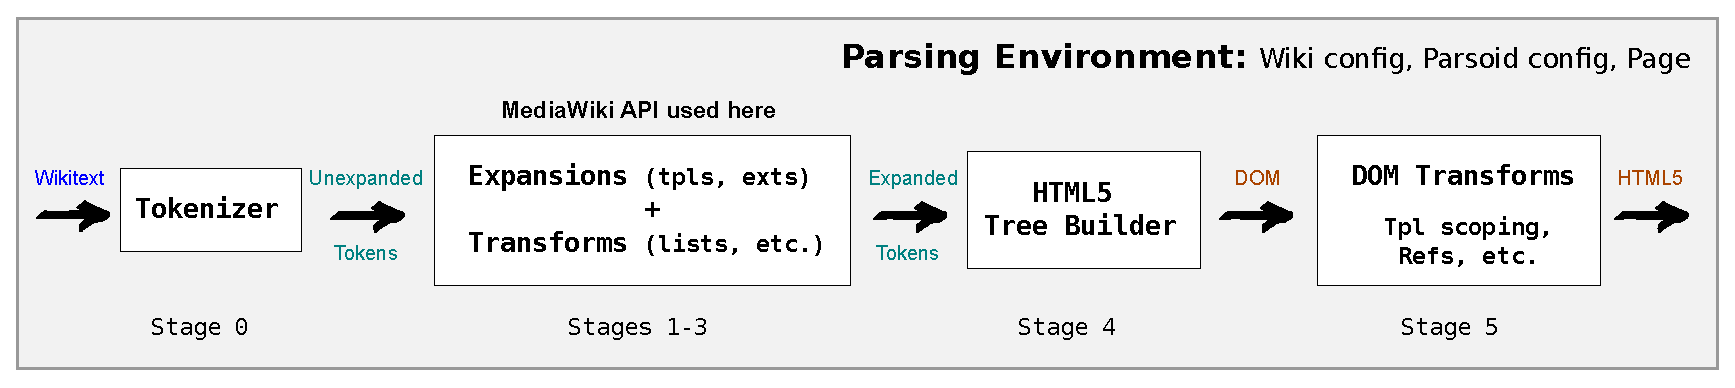
\epsfig{file=figs/parsoid.wt2html.eps,scale=0.42}\\
  {\small Wikitext to HTML (wt2html) transformation}
\end{figure}
\end{center}

\vspace{-1ex}
\begin{itemize}
  \item Use a standard HTML5 tree builder library.
  \item Use lot of tricks to detect fixup of misnested tags. \\
  {\HTML{\tt<i>X<b>Y</i></b>}} to {\HTML{\tt<i>X<b>Y</b></i><b></b>}}
  \begin{itemize}
    \item Shadow tokens added for every node found in original stream.
    \item Shadow tokens analyzed on constructed DOM to detect how misnested tags in HTML got fixed up -- analysis necessary for accuracy of mapping wikitext to DOM.
  \end{itemize}
  \item PHP parser relies on {\tt{\color{Mahogany} Tidy}} to fixup misnested tags -- causes Parsoid and PHP parser output to occasionally differ.
\end{itemize}

\end{frame}

%--- DOM transformations ---
\section{Parsoid pipeline: Stage 5: DOM transformations}

\begin{frame}{Stage 5: DOM transformations}
\vspace*{-0.3in}
\begin{center}
\begin{figure}
  \hspace*{-0.3in}
  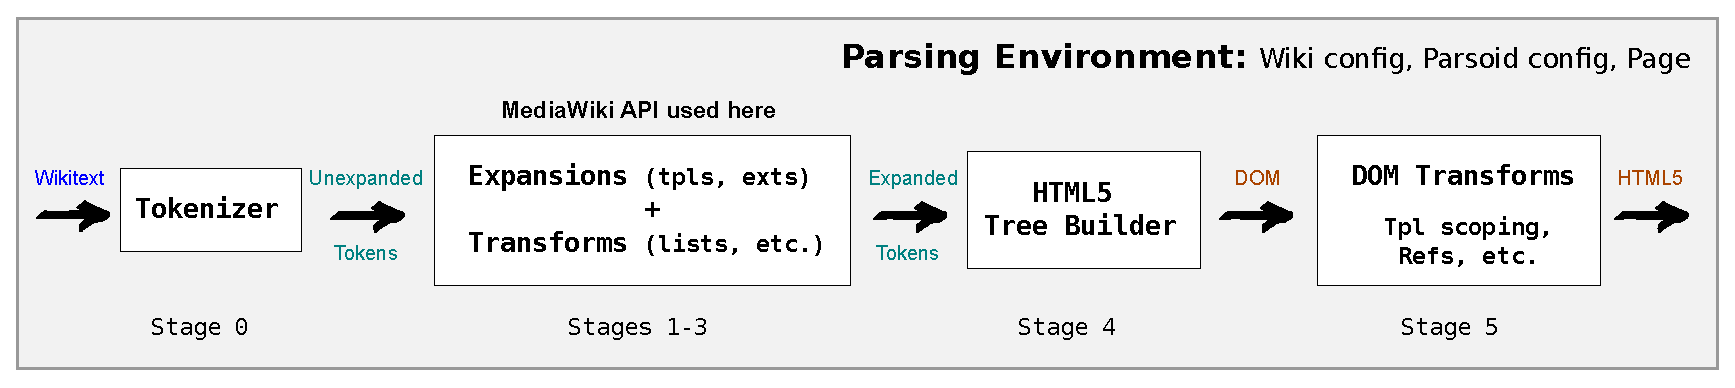
\epsfig{file=figs/parsoid.wt2html.eps,scale=0.42}\\
  {\small Wikitext to HTML (wt2html) transformation}
\end{figure}
\end{center}

\only<2>{
\begin{itemize}
  \small
  \item DOM still needs lot of fixup (ex: template scoping).
  \item DOM's tree structure $\Rightarrow$ simpler \& robust algorithms.
  \item Several passes transform the DOM.
\end{itemize}
}
\only<3> {
\begin{enumerate}
  \small
  \item Mark fostered content (Quite important!)
  \item {\color{gray}Mark HTML5 builder fixups}
  \item Map WT substrings to DOM subtrees (DSR computation)
  \item Demarcate template scopes (Template encapsulation)
  {\color{gray}
  \item Handle link prefixes/trails
  \item Generate references (Parsoid's native Cite impl)
  \item Handle LI-hack, templated table cell attributes
  }
\end{enumerate}
}

\end{frame}

\subsection{Marking fostered content}

% -- Fostered content --
\begin{frame}{DOM Pass: Marking fostered content}

\only<1>{
{\bf Fostered Content??}
\begin{itemize}
\item Fostered content = content in {\HTML{\tt<table>}}s that is badly nested and get adopted by a foster parent outside the table. \\
Example:{\HTML{\tt <table>{\color{red}foo}<tr><td>bar</td></table>}} \\
becomes:{\HTML{\tt {\color{red}foo}<table><tr><td>bar</td></table>}}
\item This is part of the HTML5 spec -- not something that Parsoid does.
\item Sometimes, partial template content gets moved out.
\end{itemize}
}

\only<2>{
{\bf Q. Why is this a problem? A. Breaks content ordering}
\begin{itemize}
\item Before this was fixed in Parsoid, this would not round-trip :
\begin{columns}[c]
  \small
  \begin{column}{0.35\textwidth}
    \begin{wikitext}
    \{|\\
    |- fostered content\\
    | foo\\
    |\}
    \end{wikitext}
  \end{column}
  \begin{column}{0.15\textwidth}
    round trips to
  \end{column}
  \begin{column}{0.35\textwidth}
    \begin{wikitext}
    fostered content\\
    \{|\\
    | foo\\
    |\}
    \end{wikitext}
  \end{column}
\end{columns}
\item Interferes with ability to map wikitext strings to generated DOM nodes.
\item When partial template content gets moved out, messes with template scoping.
\item Used to cause more serious corruption (ex: content duplication) when these pages were serialized back.
\end{itemize}
}

\only<3>{
{\bf Basic idea$^{*}$ behind solving this:}
\begin{itemize}
\item This pass adds markers before every table.
\item This effectively creates a "foster box" between the marker and the table -- i.e. content found between those two tags is fostered content.
\item Later DOM passes now ignore fostered content in their analysis.
\item Serializer relies on fostered content markers to avoid corruption.
\end{itemize}
\vspace{2ex}
{\footnotesize $*$ Caveat: Has to deal with other edge cases and fixups.}
}

\end{frame}

\subsection{DSR computation}

% -- DSR computation --
\begin{frame}{DOM Pass: DSR computation}

\only<1>{
DSR = DOM Source Range
\begin{itemize}
\item Assigned to every node in a DOM.
\item 4-tuple: [start, end, start-tag-width, end-tag-width]
\item Maps wikitext.substring(start,end) to a DOM node. \\
{\WT "foo"} will parse to {\HTML{\tt <i>foo</i>}} and
{\tt <i>}.dsr = [0,7,2,2] \\
{\WT {\tt<i>foo</i>}} will parse to {\HTML{\tt <i>foo</i>}} and
{\tt <i>}.dsr = [0,10,3,4] \\
\item Accuracy critical for selective serialization since it simply emits wikitext.substring(start,end) for unmodified DOM nodes.
\end{itemize}
}
\only<2>{
\begin{columns}
\setlength{\topsep}{0pt}
\setlength{\partopsep}{0pt}
\hspace*{-0.4in}
  \begin{column}{0.4\textwidth}
    \begin{figure}
      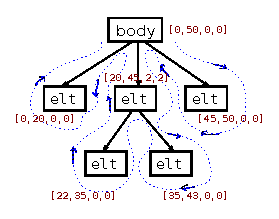
\epsfig{file=figs/dsr.algo.eps,scale=1.4}\\
    \end{figure}
  \end{column}

\hspace{1ex}

  \begin{column}{0.5\textwidth}
    \begin{itemize}
      \small
      \item DSR algo walks the DOM backward.
      \item Has a forward pass across siblings in addition at every level.
      \item Uses knowledge of wikitext and source wikitext position annotations from the tokenizer.
      \item Required us to fix other transformations, worry about newlines, etc.
      \item Uses redundant information to detect inconsistencies.
    \end{itemize}
  \end{column}
\end{columns}
}

\end{frame}

\subsection{Template Encapsulation}

\begin{frame}{DOM Pass: Template Encapsulation/Scoping}

\begin{itemize}
  \item For clients like the VisualEditor, template output cannot be directly edited and should be edit-protected.
  \item For common transclusion scenarios, output of a single transclusion can be mapped to a forest of DOM trees. \\
  Example: {\WT{\tt\{\{echo|foo\}\}}} maps to {\HTML{\tt <span..>foo</span>}}
  \item Not true in the general case. Ex: Succession box templates ({\WT \{\{s-start\}\}, ... \{\{s-end\}\}} and other such family of templates).
\end{itemize}
{\bf \small This pass associates a forest of adjacent DOM trees with a section of wikitext which includes one or more transclusions.}

\only<2>{
\begin{columns}[c]
\small
\setlength{\topsep}{0pt}
\setlength{\partopsep}{0pt}
  \begin{column}{0.20\textwidth}
    \begin{wikitext}
    \{\{s-start\}\}\\
    ... \\
    \{\{s-end\}\}\\
    \end{wikitext}
  \end{column}

  \begin{column}{0.15\textwidth}
    maps to
  \end{column}

  \begin{column}{0.65\textwidth}
    \begin{html}
    <table class="wikitable succession-box" \\
    {\bf about="\#mwt1" \\
    typeof="mw:Transclusion"\\
    data-mw=".."} ...>\\
    ...\\
    </table>
    \end{html}
  \end{column}
\end{columns}
}

\end{frame}

\begin{frame}{DOM Pass: Template Encapsulation/Scoping}

{\bf Algorithm outline}
\begin{itemize}
  \item Search for {\TOK{\tt<tpl-start>}} and {\TOK{\tt<tpl-end>}} markers and construct a set of DOM ranges (start and end DOM nodes that contain output of every transclusion).
  \uncover<2> {
  \item Merge overlapping and nested ranges.
  \item For every range, set up about id, typeof, and data-mw.
  }
\end{itemize}

\begin{columns}[c]
\small
\setlength{\topsep}{0pt}
\setlength{\partopsep}{0pt}
\uncover<1-2> {
  \begin{column}{0.4\textwidth}
  \hspace{-0.2ex}
  \begin{figure}
    
\epsfig{file=figs/template_scope.ex1.eps,scale=1.6}
  \end{figure}
  \end{column}
}

\uncover<2> {
  \begin{column}{0.6\textwidth}
  \begin{figure}
    
\epsfig{file=figs/template_scope.ex2.eps,scale=1.2}
  \end{figure}
  \end{column}
}
\end{columns}
\end{frame}

\section{Summary}

% ---- END ----
\begin{frame}{Summary}
\begin{itemize}
\item Generating html from wikitext is a fairly involved process.
\item Roundtripping and editablity requirements are new when compared to the PHP parser and complicates parsing.
\item Individual algorithms and solutions are mostly straightforward.
\item But, lot of individual components and details to get right.
\end{itemize}
\end{frame}

% ---- END ----
\begin{frame}

\vspace{10ex}
\begin{center}
\LARGE
Thank you! \\
Questions?
\end{center}

\end{frame}

\end{document}
